
%\noindent
\justifying
\setlength{\parskip}{1em}


There have been numerous amounts of research in the field of domain adaptation. Several variants of \acp{GAN} are evolved over the years to resolve various problems. Especially the image-to-image translation methods are improved significantly. This chapter aims to discuss different image-to-image translation methods. Also, a brief comparison upon existing methods carried out in section \ref{rwdiscussion}. Lastly, section \ref{rwconclusion} concludes the motivation behind choosing a particular approach.



\section{Literature Survey}\label{LiteratureSurvey}




Ian J. Goodfellow et al.\cite{goodfellow2014generative} proposed a framework of \acp{GAN} in which two models are simultaneously trained. A generative model that captures the data distribution, and a discriminative model that estimates the probability that a sample came from the training data rather than a generative model. The training procedure for a generative model is to maximize the probability of a discriminative model making a mistake. Basically, the generator learns to generate plausible data. The discriminator learns to distinguish the generator's fake data from real data. The discriminator penalizes the generator for producing implausible results. When training begins, the generator produces fake data, and the discriminator quickly learns to tell that it's fake and the generator penalized to produce plausible results. As training progresses, the generator gets closer to producing output that can fool the discriminator. Finally, if generator training goes well, the discriminator gets worse at telling the difference between real and fake. At the end of the training, eventually, we have a generator model which produces plausible results which are similar to real data. Authors have trained \ac{GAN} an a range of datasets including MNIST \cite{726791}, the Toronto Face Database (TFD) \cite{susskind2010toronto}, and CIFAR-10 \cite{krizhevsky2009learning}. Also compared against already existing methods like DBN \cite{bengio2012better}, Stacked CAE \cite{bengio2012better}, and Deep GSN \cite{bengio2014deep} . The authors do not claim that the samples generated by \acp{GAN} are better than samples generated by already existed methods. Authors believe that these samples are at least competitive with the better generative models in the literature and highlight the potential of the generative adversarial framework. The advantage of using \acp{GAN} is primarily computational. Adversarial models may also gain some statistical advantage from the generator network not being updated directly with data examples, but only with gradients flowing through the discriminator using backpropagation. Special care should be taken during training the \acp{GAN}, the generator must not be trained too much without updating the discriminator, to avoid the Helvetica Scenario \cite{manisha2019generative} in which the generator collapses to produce the same output (or a small set of outputs) over and over again. Usually, \acp{GAN} should produce a wide variety of outputs. The Helvetica Scenario is also called Mode Collapse \cite{thanhtung2020catastrophic}.
\begin{figure}
        \begin{center}
 	    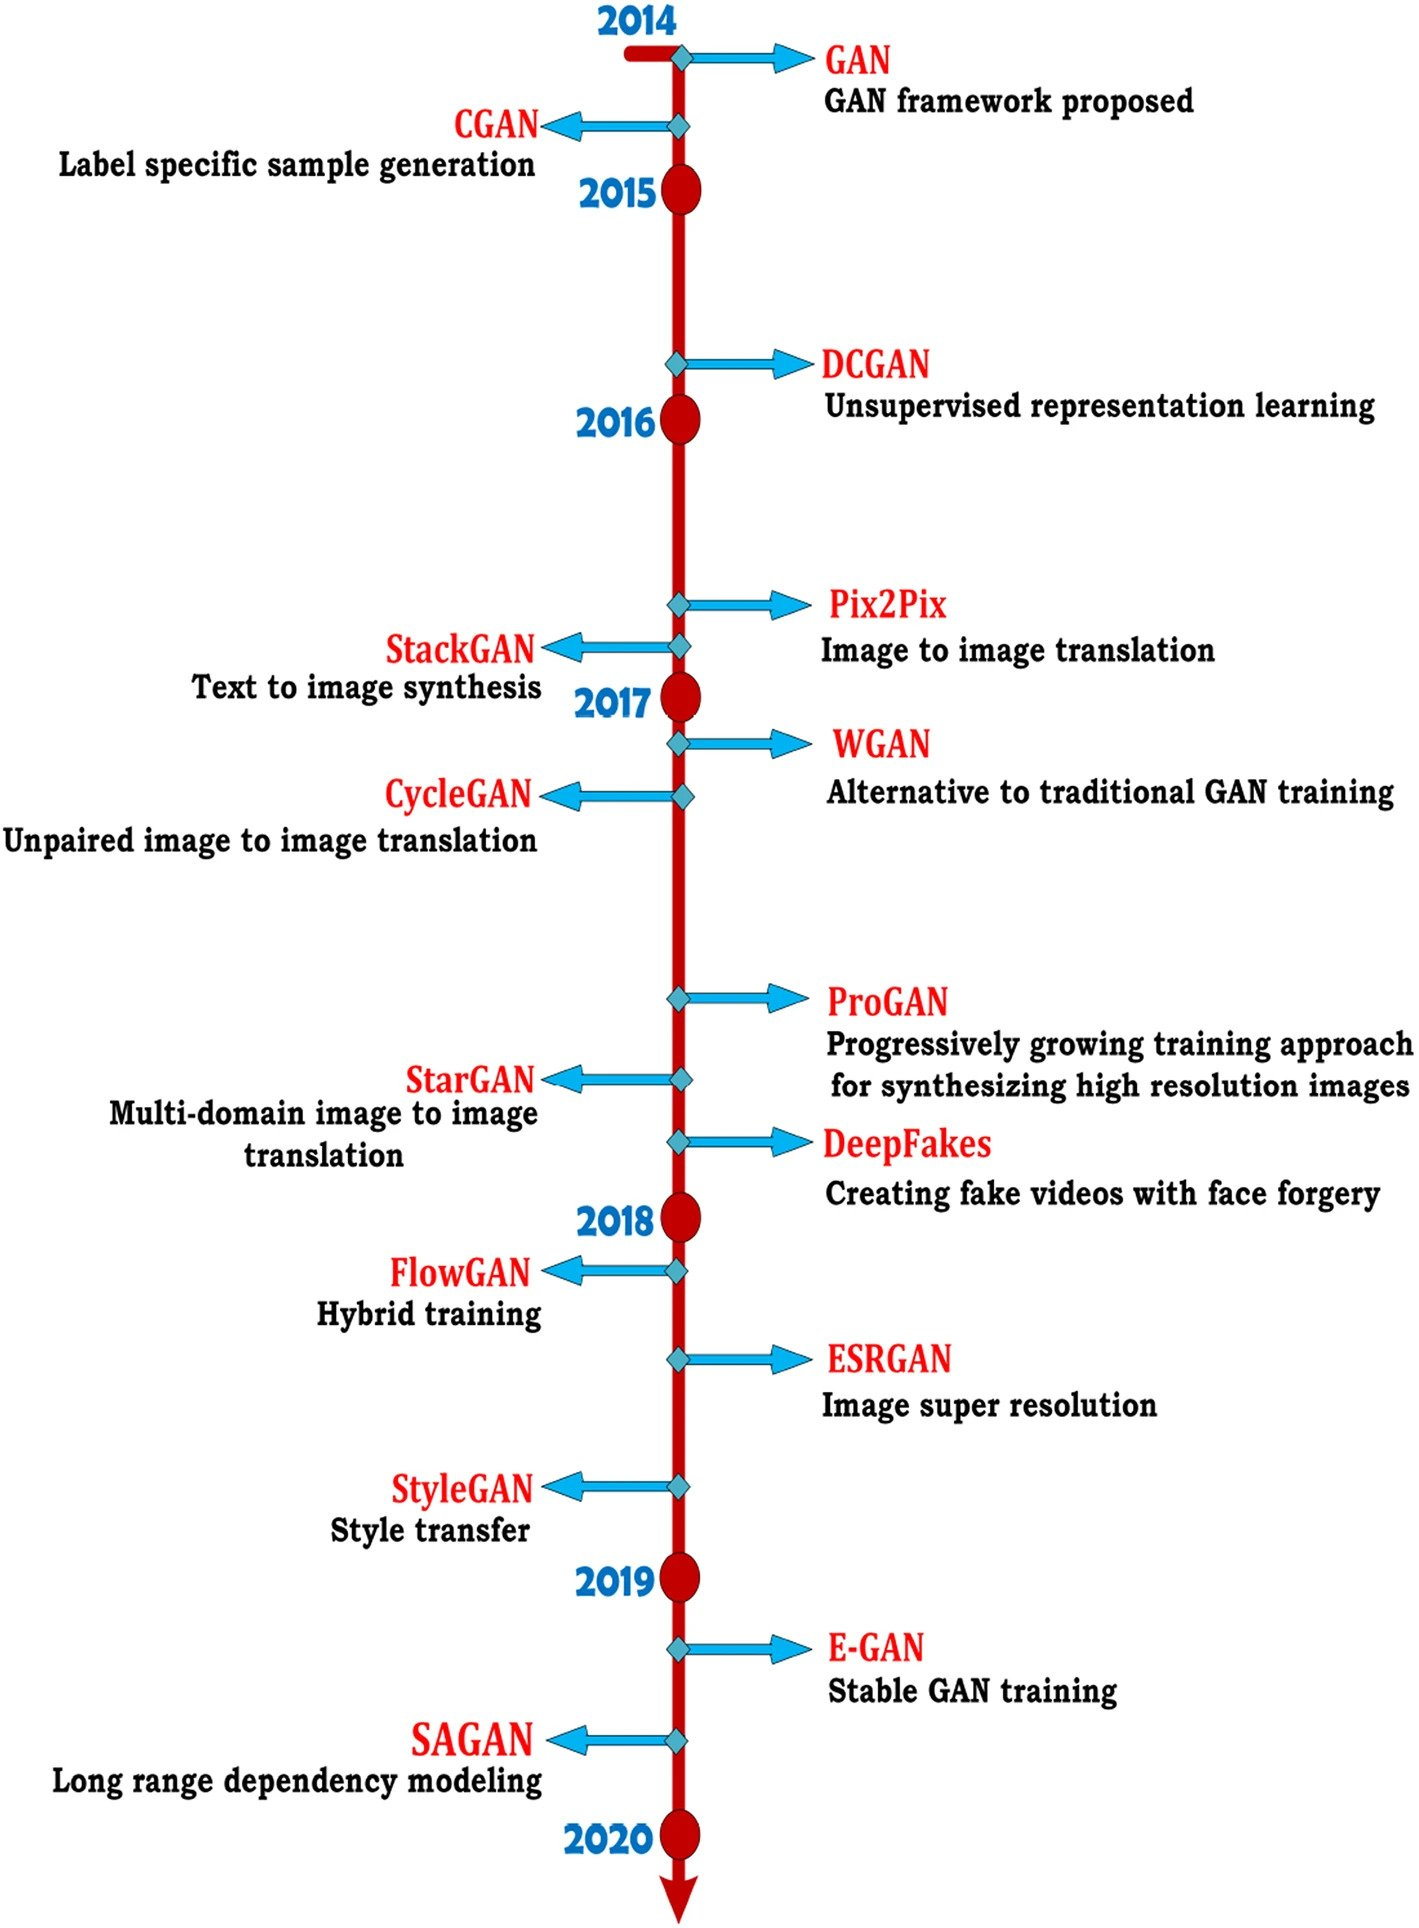
\includegraphics[scale=0.25]{images/GANEvolution.jpg}
	    \caption[Evolution of \acp{GAN} Over the Years.]{Evolution of \acp{GAN} Over the Years \cite{PavanKumar.2021}.}
	    \label{fig:GANEvolution}
	    \end{center}
\end{figure}



Xudong Mao et al.\cite{mao2017squares} proposed another variant of \acp{GAN} called \acp{LSGAN}. The Regular GANs hypothesize the discriminator as a classifier with the sigmoid cross-entropy loss function. However, they found that the cross-entropy loss function may lead to the vanishing gradients problem during the learning process. To overcome such a problem, the authors proposed the \acp{LSGAN} which adopts the least-squares loss function for the discriminator. The least-squares loss function penalizes the fake samples and forces the generator to generate samples toward the decision boundary. The authors evaluated \acp{LSGAN} using two datasets LSUN \cite{yu2016lsun} and HWDB1.0 (Handwritten Chinese Character Dataset) \cite{6065551}. When trained on the LSUN dataset \cite{yu2016lsun} they observed, the images generated by \acp{LSGAN} are of better quality than the ones generated by the two baseline methods, DCGANs \cite{radford2016unsupervised} and EBGANs \cite{zhao2017energybased}. Also, when trained on the Handwritten Chinese Character Dataset, the generated characters were readable and clear. Another experiment was conducted to evaluate the stability of \ac{LSGAN} on a Gaussian mixture distribution dataset, which is designed in literature \cite{metz2017unrolled}. They train \acp{LSGAN} and regular \ac{GAN} on a 2D mixture of 8 Gaussian datasets using a simple architecture, where both the generator and the discriminator contain three fully-connected layers. It is observed that regular \acp{GAN} suffer from mode collapse. \acp{GAN} generate samples around a single valid mode of the data distribution. But \acp{LSGAN} learn the Gaussian mixture distribution successfully. In this paper, numerous comparison experiments for evaluating the stability are conducted and the results demonstrate that \acp{LSGAN} can generate higher quality images than regular \acp{GAN}, DCGANs \cite{radford2016unsupervised}, and EBGANs \cite{zhao2017energybased} and perform more stable than regular \acp{GAN} during the learning process.


Phillip Isola et al.\cite{isola2018imagetoimage} proposed \acp{cGAN} as a generic solution to numerous image-to-image translation problems. The authors wanted to provide a single solution for multiple types of image-to-image translation problems. For example, synthesizing photos from label maps \cite{cordts2016cityscapes}, reconstructing objects from edge maps \cite{zhu2018generative} \cite{6909426} , and colorizing images. \acp{cGAN} not only learn the mapping from input image to output image, but also learn a loss function to train this mapping. This makes it possible to apply the same generic approach to problems that traditionally would require very different loss formulations. Authors implemented \ac{cGAN} and released it as the pix2pix software to solve distinct image-to-image translation problems. This software is popular among a large number of internet users, many of them are artists, because of its wide applicability and ease of adoption without the need for parameter tweaking. In \ac{cGAN} the generator uses U-Net-based architecture \cite{ronneberger2015unet}, the U-Net is an encoder-decoder with skip connections between mirrored layers in the encoder and decoder stacks. The discriminator uses a convolutional PatchGAN classifier \cite{li2016precomputed}, which only penalizes structure at the scale of image patches. Unlike unconditional GANs, both the generator and discriminator observe the input images. Authors performed multiple experiments during ablation studies using evaluation metrics like, \ac{AMT} perceptual study, FCN-Score, and semantic segmentation metrics. They found that L1 distance loss encourages less blurring compared to the L2 distance loss. Also combining L1 Loss and \ac{cGAN} (L1 + \ac{cGAN}) generates better results compared to combining Unconditional \ac{GAN} and L1 Loss ((L1 + \ac{GAN})). The \ac{cGAN} appears to be more effective on the problem where the output is highly detailed or photographic. The pix2pix software code is available at \href{https://github.com/phillipi/pix2pix.}{GitHub}. In figure \ref{fig:CGAN} the mapping from edges \textrightarrow photo transformation illustrated, and both generator and discriminator are conditioned on auxiliary information like input edge map.



\begin{figure}[H]
        \begin{center}
 	    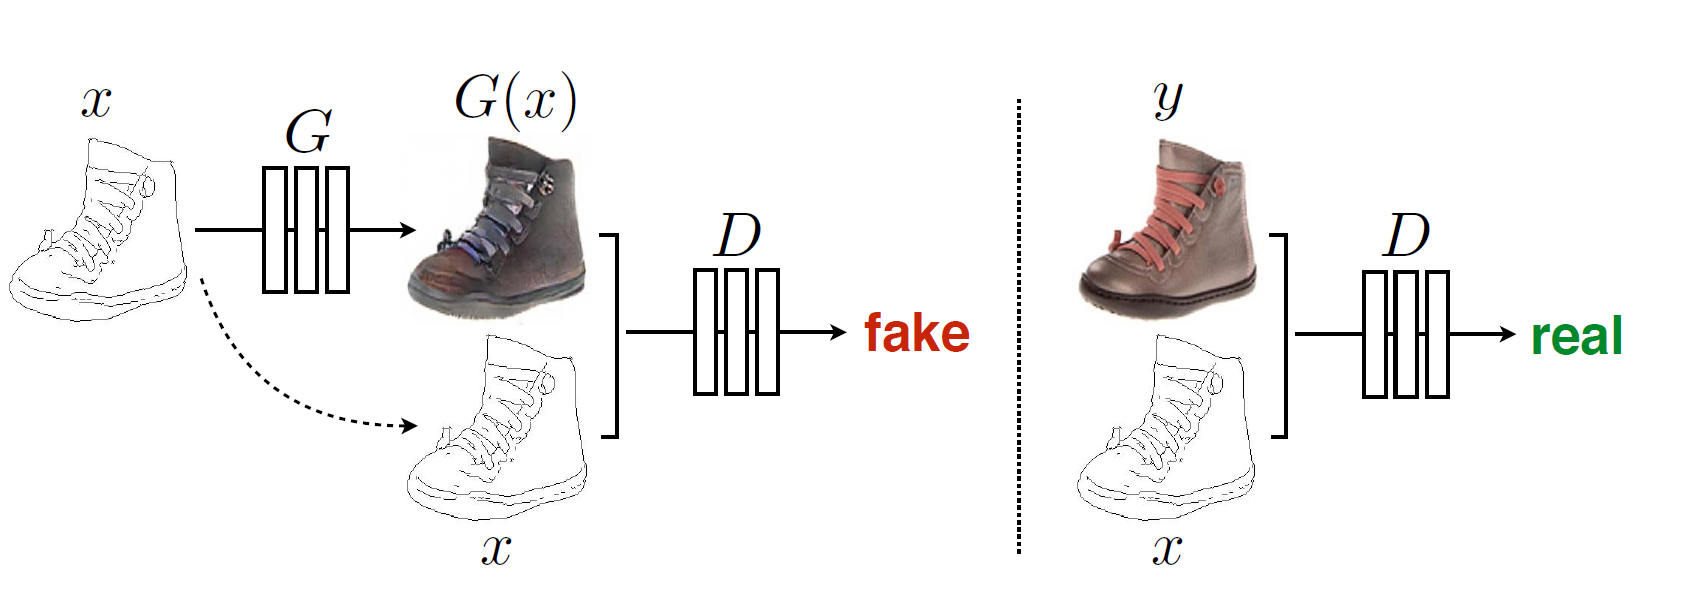
\includegraphics[scale=0.30]{images/CGAN.png}
	    \caption[Illustration of training a \ac{cGAN} to map edges \textrightarrow photo transformation.]{Illustration of training a \ac{cGAN} to map edges \textrightarrow photo transformation. Unlike unconditional \acp{GAN} both discriminator and generator observe the input edge map \cite{isola2018imagetoimage}.}
	    \label{fig:CGAN}
	    \end{center}
\end{figure}




Taesung Park et al.\cite{park2020contrastive} proposed a framework for encouraging content preservation in unpaired image-to-image translation problems by maximizing the mutual information between input and output with patchwise contrastive learning \cite{oord2019representation}. In the patchwise contrastive learning for image-to-image translation, a generated output patch should appear closer to its corresponding input patch in comparison to other random patches present in the same input. To achieve patchwise contrastive learning, drawing patches internally from within the input image, rather than externally from other images in the dataset, forces the patches to better preserve the content of the input. This method requires neither a memory bank nor specialized architecture. The authors demonstrated that the framework enables one-sided translation in the unpaired image-to-image translation setting while improving quality, consuming less memory, and reducing training time. They call this approach \ac{CUT}. Since contrastive representation is formulated within the same image, this method can even be trained on single images, where each domain is having only a single image. The several prior methods like \ac{CycleGAN} \cite{zhu2020unpaired}, \ac{MUNIT} \cite{liu2018unsupervised}, \ac{DRIT} \cite{lee2019drit}, and \ac{GCGAN} \cite{fu2018geometryconsistent} were unable to achieve significant results compared to the \ac{CUT} method, on other hand, it often produced higher quality images and more accurate generations with light footprint in terms of training speed and GPU memory usage. Since \ac{CUT} method is one-sided, it is memory efficient and faster compared to prior baselines. The evaluation metrics like \ac{FID} \cite{heusel2018gans} and semantic segmentation scores are used to compare the quality of generated images using \ac{CUT} method. Furthermore, the authors also introduced faster and lighter variant \ac{FastCUT}. \ac{FastCUT} also produces competitive results with even lighter computation cost of training. The code and models for \ac{CUT} are available at \href{https://github.com/taesungp/contrastive-unpaired-translation}{GitHub}.


\begin{figure}[H]
        \begin{center}
 	    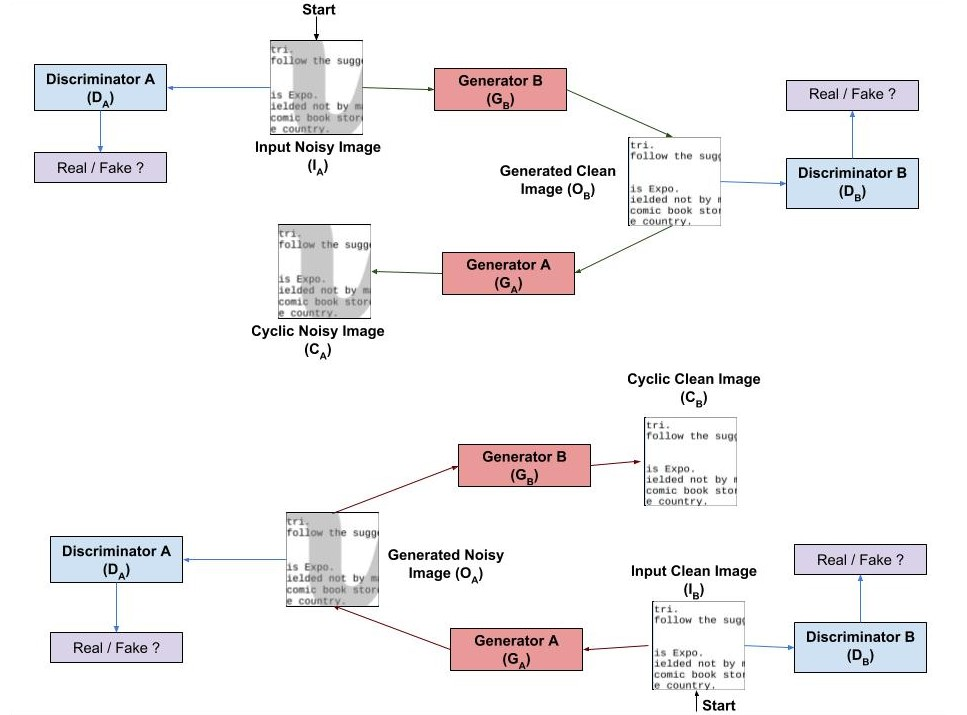
\includegraphics[scale=0.60]{images/LearningToClean.jpg}
	    \caption[Illustration of \ac{CycleGAN} transforming the noisy document images into clean document images. and vice versa.]{Illustration of CycleGAN transforming the noisy document images into clean document images. The generators $G_A$ and $G_B$ are responsible for the mapping of noisy images to clean images using cycle-consistency loss \cite{zhu2020unpaired}. And the two discriminators $D_A$ and $D_B$ rejects samples generated by $D_A$ and $D_B$ acting like an adversary \cite{sharma2019learning}.}
	    \label{fig:LearningToClean}
	    \end{center}
\end{figure}



Monika Sharma et al.\cite{sharma2019learning} is addressing a problem in the scanning process that often results in the introduction of salt and pepper noise, blur due to camera motion, or shake, water markings, coffee stains, wrinkles, or faded data. These artifacts pose many readability challenges to current text recognition algorithms and significantly degrade their performance. So, the existing denoising techniques require a dataset comprising of noisy documents paired with cleaned versions of the same document. However, very often in the real world, such a paired dataset is not available to train a model to generate clean documents from noisy versions. Hence, the authors proposed to use \ac{CycleGAN} because it is known to learn a mapping between the distributions in the absence of paired training dataset. Using \ac{CycleGAN}, noisy document images transformed into denoised and clean document images to achieve image-to-image translation. They have compared the performance of \ac{CycleGAN} for document cleaning tasks with a \ac{cGAN} by training them over the same dataset. The only difference was \ac{CycleGAN} trained using unpaired images and \ac{cGAN} trained using the paired images. They have used \ac{PSNR}\footnote{Peak Signal-to-Noise Ratio: \url{http://www.ni.com/white-paper/13306/en/} last access: 31.03.2021.} as a evaluation metric to evaluate the quality of transformed denoised images. Several experiments were performed on 4 separate document public document datasets, one each for background noise removal, deblurring, watermark removal, and defading. Finally, they illustrate that \ac{CycleGAN} learns a more robust mapping from the space of noisy to clean documents compared to \ac{cGAN}. The complete architecture of \ac{CycleGAN} for denoising documents illustrated in figure \ref{fig:LearningToClean}.


\begin{figure}[H]
        \begin{center}
 	    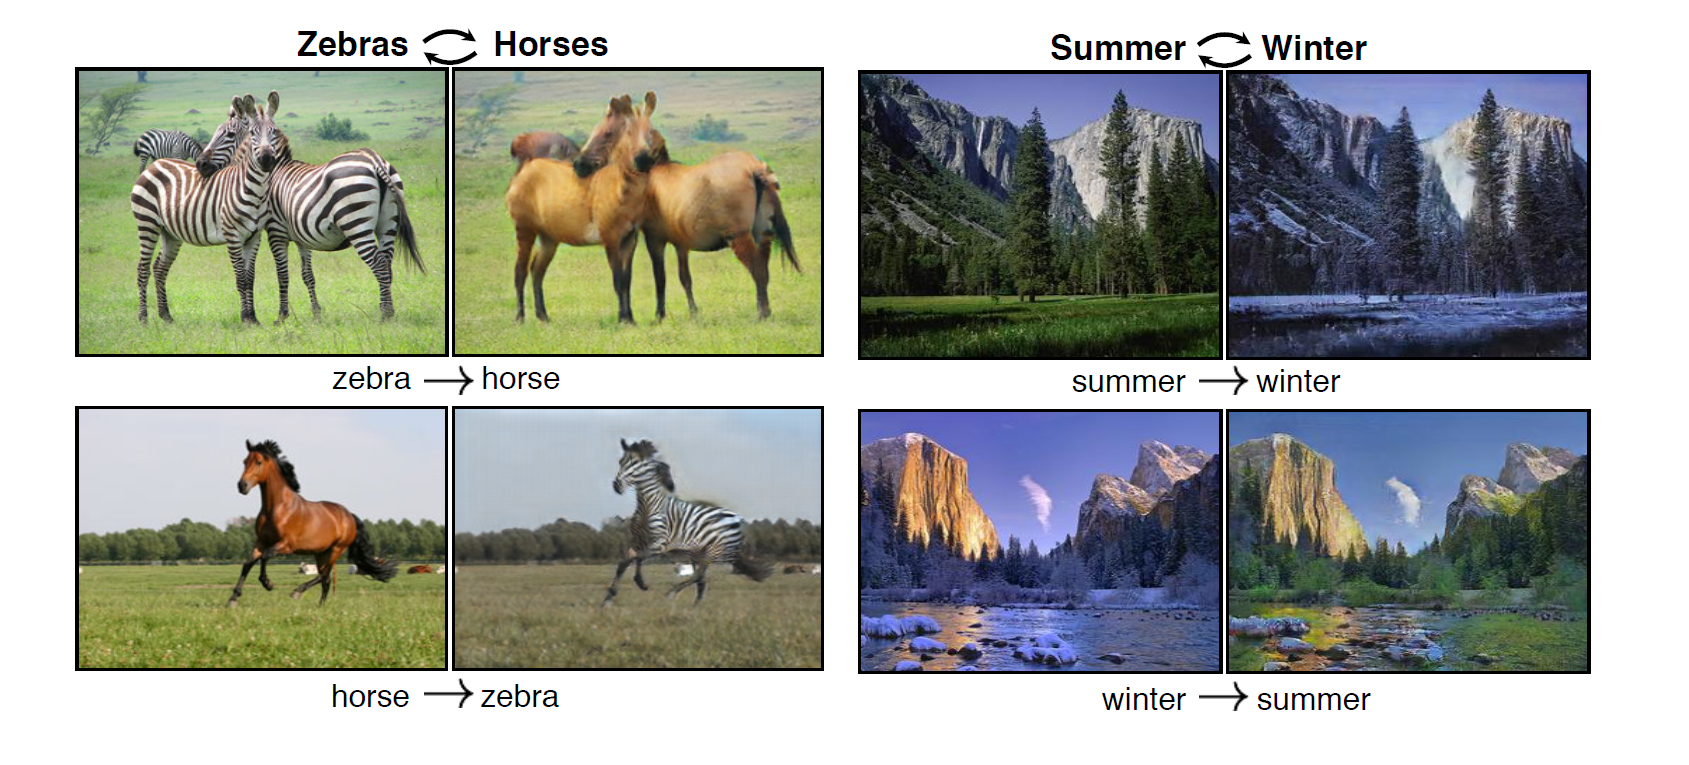
\includegraphics[scale=0.35]{images/CycleGANExamples.png}
	    \caption[Illustration of \ac{CycleGAN} transforming an image from one into the other and vice versa.]{Illustration of \ac{CycleGAN} transforming an image from one into the other and vice versa. For example, zebra image transformed into horse image, and vice versa. The view of Yosemite mountains in summer transformed into winter, and vice versa \cite{zhu2020unpaired}.}
	    \label{fig:CycleganExamples}
	    \end{center}
\end{figure}



Chris Tensmeyer et al.\cite{8978087} realized solving binarization tasks using deep learning models is very challenging. It is due to the lack of large quantities of labeled data available to train such models. They also mention there have been efforts to create synthetic data for binarization using image processing techniques but, they generally lack realism. In this paper, the authors proposed a method to produce realistic synthetic data using an adversarially trained image translation model. They extended the popular \ac{CycleGAN} model to be conditioned on the ground truth binarization mask as it translates images from the domain of synthetic images to the domain of real images. They have found that modifying the discriminator to condition on the binarization \ac{GT} leads to increased realism and better agreement between the \ac{GT} and the produced image. They called the proposed model DGT-CycleGAN. Also shown DGT-CycleGAN model produces more realistic synthetic data. They validated their approach by pretraining deep networks on realistic synthetic datasets generated by DGT-CycleGAN, \ac{CycleGAN}, and image compositing. They evaluate both pretrained only and finetuned models on each of the \ac{DIBCO} datasets. They have concluded that pretraining deep neural networks on the more realistic synthetic data generated using DGT-CycleGAN lead to better predictive performance both before and after finetuning on real data.



Jun-Yan Zhu et al.\cite{zhu2020unpaired} proposed a modified version of \ac{GAN} which is the state-of-the-art method for the image-to-image translation that can transform the images from source domain $X$ to target domain $Y$ in the absence of paired training dataset. This method can learn to capture special characteristics of one image collection and figuring out how these characteristics could be translated into the other image collection, all in the absence of any paired training examples. This modified version of \ac{GAN} is called \ac{CycleGAN}. In this method, the goal is to learn a mapping $G\ \colon X \rightarrow Y$ such that the distribution of images $G(X)$ is indistinguishable from the distribution $Y$ using an adversarial loss. Because this mapping is highly under-constrained and coupled with an inverse mapping $F\ \colon Y \rightarrow X$ to introduce a cycle consistency loss to enforce $F(G(X))\approx X$ and vice versa. Along with an adversarial loss and cycle consistency loss, this work also introduces identity mapping loss which helps to preserve the colour of input images. Authors considered evaluation metrics like \ac{AMT} perceptual studies, FCN-score \cite{isola2018imagetoimage}, and semantic segmentation metrics to compare the quality of generated images against other baseline. The several prior methods like Bi-GAN/ALI [\cite{donahue2017adversarial}, \cite{dumoulin2017adversarially}], CoGAN \cite{liu2016coupled}, SimGAN \cite{shrivastava2017learning} were unable to achieve compelling results. The \ac{CycleGAN} method, on other hand, can produce images that are often of similar quality to the fully supervised pix2pix \cite{isola2018imagetoimage}. Authors provide both \href{https://github.com/junyanz/pytorch-CycleGAN-and-pix2pix}{PyTorch} and \href{https://github.com/junyanz/CycleGAN}{Torch} implementations. In figure \ref{fig:CycleganExamples} examples of \ac{CycleGAN} transforming an image from one into the other and vice versa illustrated.



\section{Discussion}\label{rwdiscussion}
Over the years, \acp{GAN} have evolved to solve different kinds of problems. The evolution of the \acp{GAN} is illustrated in the figure \ref{fig:GANEvolution} using a timeline diagram. \acp{GAN} suffer from unstable training, vanishing gradients problem, and mode collapse. Consequently, Martin Arjovsky et al.\cite{arjovsky2017wasserstein} proposed \ac{WGAN} to solve problems with \acp{GAN}. \acp{WGAN} improve the stability of learning, get rid of problems like mode collapse, and provide meaningful learning curves useful for debugging and hyperparameter searches. Although the implementation of \ac{WGAN} is straightforward, the theory behind it is heavy and requires some hack, for example, Weight Clipping  \cite{gulrajani2017improved}. Hence, Xudong Mao et al.\cite{mao2017squares} proposed a simple and more intuitive method compared to \ac{WGAN}, called \ac{LSGAN}. First, \acp{LSGAN} are able to generate higher quality images than regular \acp{GAN}. Second, \acp{LSGAN} perform more stable during the learning process. Moreover, Jun-Yan Zhu et al.\cite{zhu2020unpaired} proposed \ac{CycleGAN}. It is an unsupervised image-to-image translation approach. Compared to \acp{GAN}, \acp{CycleGAN} can deal more meticulously with the problems like unstable training, vanishing gradients problems, and mode collapse. Also, they described that \ac{CycleGAN} has outperformed existing baselines as Bi-GAN/ALI [\cite{donahue2017adversarial}, \cite{dumoulin2017adversarially}], CoGAN\cite{liu2016coupled}, and SimGAN \cite{shrivastava2017learning}. Furthermore, Monika Sharma et al.\cite{sharma2019learning} proclaimed  \ac{CycleGAN} can transform noisy document images into denoised and clean document images to achieve image-to-image translation. They have also compared the performance of the developed image-to-image application with \ac{cGAN} and demonstrated \ac{CycleGAN} had outperformed \ac{cGAN}. Chris Tensmeyer et al.\ \cite{8978087} proposed DGT-CycleGAN, a modified version of \ac{CycleGAN}, which is adequate to translate images from the domain of synthetic images to the domain of real images to solve binarization tasks. Moreover, Taesung Park et al.\ \cite{park2020contrastive} proposed \ac{CUT}. They have demonstrated that \ac{CUT} is a better, faster, and memory-efficient approach to perform unsupervised image-to-image translation. It has outperformed \ac{CycleGAN} \cite{zhu2020unpaired}, \ac{MUNIT} \cite{liu2018unsupervised}, \ac{DRIT} \cite{lee2019drit}, and \ac{GCGAN} \cite{fu2018geometryconsistent}. However, due to time constraints, multiple available references, and code repositories, \ac{CycleGAN} has been a choice for this thesis and research to perform unsupervised image-to-image translation.


\section{Conclusion}\label{rwconclusion}

The image-to-image translation is a class of computer vision and computer graphics problems. In which the goal is to learn the mapping between a source image and target image using a training set of aligned image pairs. Although, for many tasks, aligned or paired training data will not be available. This thesis is attempting to close a domain gap between synthetic document images and real document images in the absence of paired training data. Collecting and annotating paired document images is gruelling, time-consuming, and costly. The thesis aims to develop an image-to-image translation application to transform synthetic document images into realistic document images to perform domain adaptation, by closing the gap between synthetic data distribution and real data distribution. Ultimately, a large amount of realistic annotated set of document images can be generated using this application. Furthermore, they can be used to improve document image classification. Also, in case, if a classifier trained using such generated realistic document images, it can fasten the process of labeling the new unlabeled real document images. As per the above literature survey \cite{zhu2020unpaired} \cite{sharma2019learning} and problem statement, \ac{CycleGAN} could be a remarkable approach to transform synthetic document images into realistic document images in the absence of paired training data. Hence, in this thesis, the image-to-image translation application is realized using \ac{CycleGAN}.



%In this thesis, \ac{CycleGAN} is used to perform domain adaptation. Discussion about the loss functions has been carried out in-depth in Chapter \ref{methodology}.
%is combined with \ac{LSGAN}, in which the discriminator model is updated using a least-squares loss (L2 Loss).

%The thesis aims to develop an image-to-image translation application to transform synthetic document images into realistic document images. The thesis aims to develop an image-to-image translation application to transform synthetic document images into realistic document images to perform domain adaptation. Ultimately, a large amount of realistic annotated set of document images can be generated using this application.




